% Official VTI Research Technical Report VTI-RES-2026-01 | DOI: https://doi.org/10.5281/zenodo.24290282
\documentclass[10pt,twocolumn]{article}

\usepackage[utf8]{inputenc}
\usepackage[T1]{fontenc}
\usepackage{lmodern}
\usepackage[margin=0.72in,columnsep=0.24in]{geometry}
\usepackage{microtype}
\usepackage{amsmath,amssymb,amsfonts,amsthm,mathtools}
\usepackage{booktabs,tabularx,array,multirow}
\usepackage{enumitem}
\usepackage{xcolor}
\usepackage{tikz}
\usetikzlibrary{arrows.meta,positioning}
\usepackage[hidelinks,breaklinks=true]{hyperref}
\usepackage{url}

\newtheorem{theorem}{Theorem}
\newtheorem{proposition}{Proposition}
\newtheorem{definition}{Definition}

\definecolor{vtiblue}{RGB}{18,56,110}
\definecolor{vtislate}{RGB}{242,245,250}

\title{\vspace{-1.2em}\textbf{Cognitive Harness Engineering, Human-AI Symbiosis, and Conditional Operational Parity: A Formal Multi-Plane Architecture for High-Precision Enterprise Agentic Systems}}

\author{
  \textbf{Caio Gon\c{c}alves}\\
  \small Principal Investigator \& Chief Systems Architect, VTI Research (VTI, Brazil)\\
  \small Technical Report \texttt{VTI-RES-2026-01} $\cdot$ \url{https://projectos-system.github.io/vti-research/}
}

\date{November 2026}

\begin{document}
\maketitle

\begin{abstract}
Deploying agentic artificial intelligence across high-liability institutional domains---spanning federal and state tax advisory, corporate accounting (\texttt{IFRS/CPC}), income tax computation, value-added tax reform (\texttt{IBS/CBS}), tax substitution (\texttt{ICMS-ST}), civil and tax litigation, labor and social security compliance, autonomous software engineering, and commercial advisory surfaces---confronts a structural tension among frontier inference cost, second-order statutory omissions in compact workhorse models, and live governance of \emph{Human-in-the-Loop} symbiosis. Drawing on a controlled repeated-measures experiment ($5 \times 20 = 100$ end-to-end executions) conducted on the \textbf{Enterprise Advisory \& Commercial Agent Hub} ($\mathcal{S}_{\mathrm{Hub}}$, operating over an authentic Brazilian corpus of $374{,}252$ semantic vectors and $396{,}176$ normative acts) alongside an architectural audit of \textbf{MemoryOS} ($\mathcal{S}_{\mathrm{Mem}}$, part of \texttt{VTI OS System}) and the \textbf{Automated Regulatory Ingestion \& Editorial Auditing Platform} ($\mathcal{S}_{\mathrm{Reg}}$, monitoring $43$ daily official sources), we empirically show that scaling unconstrained internal reasoning (\texttt{reasoning.effort} from \texttt{low} to \texttt{medium} and \texttt{high}) in compact reasoning models (\texttt{Tier-W Compact Reasoning Model}, \texttt{W-Compact}) fails to remediate missing statutory \emph{mindware} and induces \textbf{\emph{Sub-Parametric Overthinking}}: under partial deterministic oracle coverage in Query 8, intermediate deliberation ($1{,}143$ hidden tokens) degraded accuracy from $20/20$ to $19/20$ by rationalizing against retrieved documentary evidence, whereas \texttt{high} effort ($36{,}593$ hidden tokens) inflated mean latency by $+76.4\%$ over \texttt{low} ($27.62\text{ s}$ vs.\ $15.66\text{ s}$) while still missing the second-order charitable immunity withholding exception in Query 7 (\texttt{CEBAS 20\%}). Grounded in Stanovich's Tripartite Theory of Mind, metabolic efficiency invariants from comparative cognitive physiology, and recent advances in \emph{Harness Engineering} and \emph{Human-AI Complementarity}, we formalize the \textbf{Cognitive Harness Parity Engine (\texttt{HPE v3.0})} across four decoupled planes and eight mathematical models (\texttt{M1--M8}): non-compensatory paired parity ($G_s = C_s T_s S_s \in \{0,1\}$, proving $n_j^* = 736$ and $1{,}125$ under Holm-7), bounded dual-exponential saturation (\texttt{M2}), residual \emph{Boost-Only} fusion with exact submodular \emph{Micro-Card} selection (\texttt{M3}), Tri-Route lexicographic routing under a Shared Monotonic Deadline and doubly robust \texttt{AIPW} auditing (\texttt{M4}), \texttt{Ed25519}/\texttt{RFC 8785 JCS} blueprint compilation across seven agent families \texttt{F1--F7} (\texttt{M5}), asynchronous bitemporal metabolism under legal partial order $\preceq_{\mathrm{jur}}$ (\texttt{M6}), constrained naturalness and \texttt{AST SSML} voice (\texttt{M7}), and Human-AI symbiosis with four in-flight revocation checkpoints \texttt{CP-1..3}, ergodic queues ($\varrho_q \le 0.80 < 1$), physical SQL ACLs under a material \texttt{Two-Person Rule}, and DAG-verified Anti-Goodhart feedback (\texttt{M8}), certified across $13$ E2E batteries (\texttt{B1--B13}).
\end{abstract}

\noindent\textbf{Keywords:} Harness Engineering; Compound AI Systems; Human-in-the-Loop Symbiosis; Stanovich Epistemic Rationality; Sub-Parametric Overthinking; Blueprint Compilation; Anti-Goodhart Governance.

\section{Introduction and Scientific State of the Art}

The transition of generative AI from open-ended chat assistants into auditable institutional infrastructure has shifted the primary locus of systems research from isolated transformer parameter counts to the coupled triad $(H_{\mathrm{op}}, m, H)$ of human specialist, language model, and external cognitive harness \cite{zaharia2024shift,khattab2024dspy,bansal2021does}. In domains governed by positive statutory law, corporate accounting standards, and commercial authority tiers---where an inverted withholding rate, reliance on a repealed norm, or an unauthorized contractual discount creates immediate liability---separating intrinsic algorithmic capacity from external deterministic scaffolding and human intentional sovereignty is foundational.

Seven research streams from 2020--2026 anchor our architecture:
\begin{enumerate}[leftmargin=*,nosep]
  \item \textbf{Harness Lifting for Compact Models:} Yang et al.\ \cite{yang2026better} demonstrated across $21$ enterprise task-model pairs that compact models collapse to $31.4\%$ when run inside frontier-oriented harnesses, yet jump to $89.7\%$ ($+58.3$ pp) at $4\%$ of frontier cost once task complexity is lifted into deterministic harness structures.
  \item \textbf{Programmatic Pipeline \& Interface Design:} Declarative compilation \cite{khattab2024dspy} and agent-computer interface engineering \cite{jimenez2024swebench,yang2024sweagent} yield $>6\times$ multipliers over identical frozen weights while compressing context usage.
  \item \textbf{Long-Context \& Unconstrained Planning Drift:} Positional degradation \cite{liu2024lost} and unconstrained reasoning chains accumulate premise drift in smaller models when intermediate steps lack deterministic external checks.
  \item \textbf{Oracle-Mediated vs.\ Intrinsic Critique:} Whereas purely internal self-correction fails to improve deductive reasoning \cite{huang2024large}, tool-interactive critique \cite{gou2024critic} and independent verification \cite{du2024improving} converge reliably.
  \item \textbf{Statutory RAG Hallucinations \& Bitemporality:} Magesh et al.\ \cite{magesh2025hallucination} showed that leading legal RAG tools hallucinate in $17\%$--$33\%$ of queries involving normative hierarchy, bitemporal validity \cite{jensen1999temporal,kulkarni2012temporal}, or second-order statutory exceptions.
  \item \textbf{Risk-Aware Cascades \& Selective Labels:} Cost-saving cascades \cite{chen2023frugalgpt,ong2025routellm} require non-compensatory tail bounds and doubly robust counterfactual estimation \cite{lakkaraju2017selective,robins1994estimation} to avoid silent false negatives.
  \item \textbf{Human-AI Complementarity \& Anti-Goodhart Governance:} Complementary team performance ($\operatorname{Perf}(H_{\mathrm{op}}+M) > \max\{\operatorname{Perf}(H_{\mathrm{op}}),\operatorname{Perf}(M)\}$) requires bounded human supervisory load \cite{parasuraman2000model,amershi2019guidelines,wilder2020learning,bansal2021does} and structural root-cause remediation rather than database hot-patching to defeat Goodhart's Law \cite{goodhart1975problems,strathern1997improving}.
\end{enumerate}

Grounded in Stanovich's Tripartite Theory of Mind \cite{stanovich2009what,stanovich2011rationality,stanovich2016rationality,evans2013dual,deneys2023advancing}, scaling \texttt{reasoning.effort} expands serial simulation in the \emph{Algorithmic Mind}, but cannot synthesize missing declarative/procedural \emph{Mindware}, replace conflict monitoring in the \emph{Reflective Mind}, or supersede \emph{Human Intentional Sovereignty}.

\subsection{Epistemological Scope of the Physiological Analogy and System Standardization}

Cortical signaling operates within a tight $\sim 20\text{ W}$ energy budget via selective gene expression, spinal/cerebellar reflex arcs, dorsal anterior cingulate (\texttt{dACC}) conflict monitoring prior to prefrontal recruitment \cite{attwell2001energy,botvinick2001conflict,baddeley2000episodic}, and complementary hippocampal-neocortical learning systems \cite{mcclelland1995why,gutierrez2024hipporag}. In this work, physiology serves strictly as: (i) a modular decomposition heuristic, (ii) an internal architectural taxonomy, and (iii) a source of resource-isolation invariants. We claim zero biological equivalence, never substitute metaphor for proof, and keep observability projection strictly unidirectional with zero anatomical terms in schemas, APIs, or prompts.

\paragraph{Evaluated Enterprise Ecosystems and Normalized Tiers.}
Our empirical and engineering study spans three integrated production systems: (1) \textbf{MemoryOS} ($\mathcal{S}_{\mathrm{Mem}}$, within \texttt{VTI OS System}), providing bitemporal hybrid memory and multi-model epistemic governance; (2) the \textbf{Enterprise Advisory \& Commercial Agent Hub} ($\mathcal{S}_{\mathrm{Hub}}$), serving tax, accounting, labor, and litigation advisory alongside commercial/executive agents over $374{,}252$ semantic vectors and $396{,}176$ normative acts; and (3) the \textbf{Automated Regulatory Ingestion \& Editorial Auditing Platform} ($\mathcal{S}_{\mathrm{Reg}}$), monitoring $43$ daily official Brazilian sources. Evaluated models are standardized through the enterprise AI gateway (mapping canonical plans onto OpenAI Responses API \texttt{/v1/responses} and Google GenAI \texttt{thinkingConfig}):
\begin{itemize}[leftmargin=*,nosep]
  \item \textbf{Tier-W Compact Reasoning Model (\texttt{W-Compact}):} US\$ $0.10 / 10^6$ input and US\$ $0.50 / 10^6$ public-list output tokens (US\$ $0.40 / 10^6$ contracted volume billing);
  \item \textbf{Tier-F Frontier Reasoning Model (\texttt{F-Frontier}):} US\$ $2.00 / 10^6$ input and US\$ $10.00 / 10^6$ public-list output tokens (US\$ $8.00 / 10^6$ contracted volume billing).
\end{itemize}

\begin{table*}[t]
\centering
\caption{Paired Repeated-Measures Benchmark on $\mathcal{S}_{\mathrm{Hub}}$ ($5$ Profiles $\times$ $20$ Audited Queries $= 100$ Executions).}
\label{tab:benchmark}
\footnotesize
\begin{tabularx}{\textwidth}{l c c c c r r c r}
\toprule
\textbf{Paired Profile ($n=20$)} & \textbf{Transport} & \textbf{Core Thesis} & \textbf{Q7 (\texttt{CEBAS 20\%})} & \textbf{Q8 (\texttt{FPAS 507})} & \textbf{Reason Tok.} & \textbf{Vis. Tok.} & \textbf{Mean Latency (LLM)} & \textbf{20Q Cost (65k/yr)} \\
\midrule
1. \texttt{F-Frontier} (\texttt{low}, Baseline) & \texttt{/v1/responses} & $20/20$ & Captured & $0$ err (\texttt{507}) & \emph{embedded} & $10{,}426$ & $22.99\text{ s}$ ($10.63\text{ s}$) & US\$ $0.9362$ (\$3,042.64) \\
2. \texttt{W-Compact} (\texttt{none}) & \texttt{/v1/chat/comp.} & $20/20^*$ & Omitted & $0$ err (\texttt{507}) & $0$ & $6{,}767$ & $15.23\text{ s}$ ($4.91\text{ s}$) & US\$ $0.0451$ (\$146.69) \\
\textbf{3. \texttt{W-Compact} (\texttt{low}, Optimum)} & \texttt{/v1/responses} & $\mathbf{20/20}$ & Omitted & $\mathbf{0}$ \textbf{err (\texttt{507})} & $\mathbf{1{,}311}$ & $6{,}734$ & $\mathbf{15.66\text{ s}}$ ($\mathbf{6.26\text{ s}}$) & \textbf{US\$ $\mathbf{0.0457}$ (\$148.40)} \\
4. \texttt{W-Compact} (\texttt{medium}) & \texttt{/v1/responses} & $19/20$ & Denied & \textbf{Failed (\texttt{515})} & $15{,}289$ & $6{,}942$ & $15.88\text{ s}$ ($12.48\text{ s}$) & US\$ $0.0528$ (\$171.70) \\
5. \texttt{W-Compact} (\texttt{high}) & \texttt{/v1/responses} & $20/20^{**}$ & Denied & $0$ err (\texttt{507}) & $36{,}593$ & $6{,}914$ & $27.62\text{ s}$ ($21.60\text{ s}$) & US\$ $0.0633$ (\$205.80) \\
\bottomrule
\end{tabularx}
\vspace{0.2em}
\par\raggedright\scriptsize $^*$1 syntactic truncation on Q19 ($150$ tokens). $^{**}$Residual English header (\texttt{\#\#\# Sources:}) on Q13 and latency spikes up to $55.0\text{ s}$ (Q10).
\end{table*}

\section{Precursor Empirical Evidence and Models \texttt{M1--M2}}

\subsection{Paired Benchmark ($5 \times 20 = 100$) and \emph{Sub-Parametric Overthinking}}

Table~\ref{tab:benchmark} reports our precursor repeated-measures benchmark across $N=20$ real-world Brazilian labor and social security queries. Statistically, the $100$ runs form a paired block design ($N=20$ independent query units), and under an exact one-sided $97.5\%$ Clopper--Pearson bound \cite{clopper1934use}, $0/20$ errors bounds population failure only at $p_U = 1 - 0.025^{1/20} \approx 0.1684$. Mechanistically, holding retrieved context fixed across Queries 7, 8, and 15 isolates three laws:
\begin{enumerate}[leftmargin=*,nosep]
  \item \textbf{Invariance of 2nd-Order Mindware Gaps (\texttt{Q7}):} For a charitable association hiring an autonomous contractor, the statutory bridge to conditional \texttt{CEBAS 20\%} withholding (\texttt{Art.\ 37, I, ``b'', IN RFB 2,110/2022}) was absent from lexical retrieval and \texttt{W-Compact} weights; scaling hidden tokens from $275$ (\texttt{low}) to $3{,}106$ (\texttt{high}, $35.15\text{ s}$) failed to recover it.
  \item \textbf{Sub-Parametric Overthinking (\texttt{Q8}):} On \texttt{CNAE 0910-6/00}, a 4-row pilot seed returned \texttt{UNMAPPED}. \texttt{W-Compact (low)} faithfully followed the retrieved normative opinion (\texttt{FPAS 507}), whereas \texttt{medium} ($1{,}143$ hidden tokens) over-rationalized semantically (\emph{``support implies services $\Rightarrow$ FPAS 515''}), degrading accuracy to $19/20$.
  \item \textbf{Sufficiency of Deterministic Prosthetics (\texttt{Q15}):} On \texttt{CNAE 9430-8/00}, fully covered in the local catalog across four regimes (\texttt{515, 566, 523, 639/CEBAS}), every \texttt{W-Compact} profile matched \texttt{F-Frontier} identically.
\end{enumerate}

\subsection{Model \texttt{M1}: Non-Compensatory Parity and Sample-Size Theorem}

For system $s \in \{c, f\}$ with $c=(m_{\mathrm{W}}, H_{\mathrm{HPE}})$ and $f=(m_{\mathrm{F}}, H_{\mathrm{base}})$, each evaluation yields binary blocking gates for material correctness $C_s \in \{0,1\}$, bitemporal statutory validity $T_s \in \{0,1\}$, and security/surface compliance $S_s \in \{0,1\}$ (\texttt{UNKNOWN} fails closed: $G_s=0$):
\begin{align}
G_s(q,\omega) &= C_s(q,\omega)\cdot T_s(q,t_{\mathrm{ref}},\omega)\cdot S_s(q,\omega) \in \{0,1\}, \\
V_s(q,\omega) &= \sum_{k \in \{E,F,A,U\}} \alpha_k m_{k,s}(q,\omega), \quad Q_s = G_s \cdot V_s,
\end{align}
with $\alpha_k \ge 0$, $\sum_k \alpha_k = 1$. Across domain strata $j \in \{1,\dots,J\}$, defining $p_{s,j}=\mathbb{E}_j[G_s]$, $u_{s,j}=\mathbb{E}_j[Q_s]$, and $v_{s,j}^{\cap}=\mathbb{E}_j[V_s \mid G_c=1 \land G_f=1]$, Conditional Operational Parity requires:
\begin{equation}
\begin{aligned}
\operatorname{LCB}_{1-\alpha_{G,j}}(p_{c,j}-p_{f,j}) &\ge -\delta_{\mathrm{hard},j}, \\
\operatorname{LCB}_{1-\alpha_U}(u_c-u_f) &\ge -\varepsilon_p, \quad
\operatorname{LCB}_{1-\alpha_V}(v_c^{\cap}-v_f^{\cap}) \ge -\varepsilon_{\mathrm{soft}}.
\end{aligned}
\end{equation}

\begin{theorem}[Exact Stratum Sample-Size Bound]
To certify non-inferiority margin $\delta_{\mathrm{hard},j} \in (0,1)$ at one-sided level $\alpha_{j,\mathrm{local}} \in (0,1)$ even under zero adverse discordances ($n_{01,j}=0$), independent paired sample size $n_j$ must satisfy:
\begin{equation}
n_j \ge n_j^* = \left\lceil \frac{\ln(\alpha_{j,\mathrm{local}})}{\ln(1 - \delta_{\mathrm{hard},j})} \right\rceil.
\end{equation}
\end{theorem}
\begin{proof}
When $G_{f,i}=1$ for all $i$ and $n_{01,j}=0$, the exact Clopper--Pearson upper bound \cite{clopper1934use} on $\theta_j = \mathbb{P}(G_c=0,G_f=1)$ satisfies $(1-\theta_U)^{n_j}=\alpha_{j,\mathrm{local}}$, so $\operatorname{LCB} = -(1-\alpha_{j,\mathrm{local}}^{1/n_j}) \ge -\delta_{\mathrm{hard},j} \iff n_j \ge \ln(\alpha_{j,\mathrm{local}})/\ln(1-\delta_{\mathrm{hard},j})$. For $\alpha_{j,\mathrm{local}}=0.025$ and $\delta_{\mathrm{hard},j}=0.005$, $n_j^* = \lceil 735.93 \rceil = 736$; under Holm--Bonferroni \cite{holm1979simple} across $J=7$ domains ($\alpha_{j,\mathrm{local}}=0.025/7$), $n_j^* = \lceil 1{,}124.39 \rceil = 1{,}125$.
\end{proof}

\subsection{Model \texttt{M2}: Bounded Dual-Exponential Saturation}

Let $\Omega(q,H) \in [0,1]$ be deterministic harness anchoring and $\Delta_{\mathrm{prior}}(m,q) \ge 0$ be prior divergence. With $\tau_{v,m},\tau_{d,m},\tau_{\nu,m} > 0$ and finite $A_m,B_m,\nu_m \ge 0$, net latent evidence $z_m$ and accuracy over effort $e \ge 0$ satisfy:
\begin{align}
z_m(q,e,H) &= z_{0,m} + A_m\Omega\!\left(1 - e^{-e/\tau_{v,m}}\right) \nonumber\\
           &\quad - B_m(1-\Omega)\Delta_{\mathrm{prior}}\!\left(1 - e^{-e/\tau_{d,m}}\right), \\
P_{\mathrm{correct}}(m,e,H) &= \Phi\!\left(\frac{z_m(q,e,H)}{\sqrt{1 + \nu_m(1 - e^{-e/\tau_{\nu,m}})}}\right).
\end{align}
As $e \to \infty$, $P_{\mathrm{correct}}$ converges to a strictly bounded asymptote in $(0,1)$. When syntactic verification saturates faster than associative drift ($\tau_{v,m} < \tau_{d,m}$) under $0 < \Omega < 1$, $\partial z_m/\partial e$ switches from positive near $e=0$ (\texttt{low}) to negative at intermediate $e$ (\texttt{medium}, \texttt{Q8}), whereas $\Omega \to 1$ under certified oracles eliminates $(1-\Omega)$ identically.

\section{Architectural Gap Diagnosis Across Enterprise Systems}

Forensic inspection across $\mathcal{S}_{\mathrm{Hub}}$, $\mathcal{S}_{\mathrm{Mem}}$, and $\mathcal{S}_{\mathrm{Reg}}$ exposed four systemic gaps: (1) asymmetric deterministic oracle coverage across dense statutory domains alongside first-order-only lexical retrieval; (2) blueprint replication drift lacking canonical family locks (\texttt{F1--F7}) and tool-revocation semantics; (3) multiplicative timeout amplification ($T_{\mathrm{worst}} \approx N_{\mathrm{keys}} \times \mathrm{timeoutMs} \times N_{\mathrm{providers}}$) and routing decoupled from post-RRF risk scores; and (4) $30\text{ s}$ TTL LLM caches lacking in-flight revocation checkpoints, unstructured coexistence of historical advisory replies (\texttt{P4}) with primary statutes (\texttt{P0/P1}), and the need for physical SQL ACLs, ergonomic queue bounds, and an append-only Anti-Goodhart regulatory outbox.

\begin{figure*}[t]
\centering
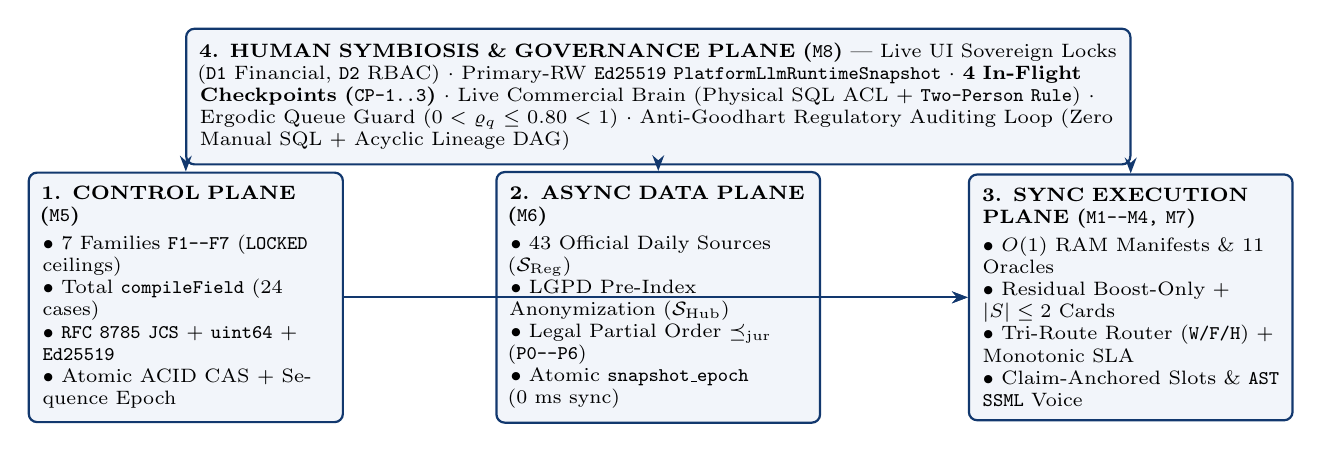
\begin{tikzpicture}[
  font=\scriptsize,
  plane/.style={draw=vtiblue, thick, rounded corners=3pt, fill=vtislate, align=left, inner sep=5pt},
  arr/.style={-{Stealth[length=2mm]}, thick, draw=vtiblue}
]
\node[plane, text width=0.96\textwidth] (hp) at (0, 2.55) {
  \textbf{4. HUMAN SYMBIOSIS \& GOVERNANCE PLANE (\texttt{M8})} --- Live UI Sovereign Locks (\texttt{D1} Financial, \texttt{D2} RBAC) $\cdot$ Primary-RW \texttt{Ed25519} \texttt{PlatformLlmRuntimeSnapshot} $\cdot$ \textbf{4 In-Flight Checkpoints (\texttt{CP-1..3})} $\cdot$ Live Commercial Brain (Physical SQL ACL + \texttt{Two-Person Rule}) $\cdot$ Ergodic Queue Guard ($0 < \varrho_q \le 0.80 < 1$) $\cdot$ Anti-Goodhart Regulatory Auditing Loop (Zero Manual SQL + Acyclic Lineage DAG)
};

\node[plane, text width=0.30\textwidth, minimum height=2.2cm] (cp) at (-6.0, 0) {
  \textbf{1. CONTROL PLANE (\texttt{M5})}\\[2pt]
  $\bullet$ 7 Families \texttt{F1--F7} (\texttt{LOCKED} ceilings)\\
  $\bullet$ Total \texttt{compileField} (24 cases)\\
  $\bullet$ \texttt{RFC 8785 JCS} + \texttt{uint64} + \texttt{Ed25519}\\
  $\bullet$ Atomic ACID CAS + Sequence Epoch
};

\node[plane, text width=0.31\textwidth, minimum height=2.2cm] (dp) at (0.0, 0) {
  \textbf{2. ASYNC DATA PLANE (\texttt{M6})}\\[2pt]
  $\bullet$ 43 Official Daily Sources ($\mathcal{S}_{\mathrm{Reg}}$)\\
  $\bullet$ LGPD Pre-Index Anonymization ($\mathcal{S}_{\mathrm{Hub}}$)\\
  $\bullet$ Legal Partial Order $\preceq_{\mathrm{jur}}$ (\texttt{P0--P6})\\
  $\bullet$ Atomic \texttt{snapshot\_epoch} ($0\text{ ms}$ sync)
};

\node[plane, text width=0.31\textwidth, minimum height=2.2cm] (ep) at (6.0, 0) {
  \textbf{3. SYNC EXECUTION PLANE (\texttt{M1--M4, M7})}\\[2pt]
  $\bullet$ $O(1)$ RAM Manifests \& 11 Oracles\\
  $\bullet$ Residual Boost-Only + $|S|\le 2$ Cards\\
  $\bullet$ Tri-Route Router (\texttt{W/F/H}) + Monotonic SLA\\
  $\bullet$ Claim-Anchored Slots \& \texttt{AST SSML} Voice
};

\draw[arr] (hp.south -| cp.north) -- (cp.north);
\draw[arr] (hp.south -| dp.north) -- (dp.north);
\draw[arr] (hp.south -| ep.north) -- (ep.north);
\draw[arr] (cp.east) -- (ep.west);
\draw[arr] (dp.east) -- (ep.west);
\end{tikzpicture}
\caption{Four-plane decoupled architecture of the \textbf{Cognitive Harness Parity Engine (\texttt{HPE v3.0})} across $\mathcal{S}_{\mathrm{Mem}}$, $\mathcal{S}_{\mathrm{Hub}}$, and $\mathcal{S}_{\mathrm{Reg}}$.}
\label{fig:architecture}
\end{figure*}

\section{Formal Architecture of \texttt{HPE v3.0} (\texttt{M3--M8})}

Figure~\ref{fig:architecture} depicts the four orthogonal planes of \texttt{HPE v3.0}.

\subsection{Model \texttt{M3}: Residual \emph{Boost-Only} Fusion, Submodular Micro-Cards, and 11 Bitemporal Oracles}

The bridge graph $\mathcal{G}_{\mathrm{bridge}}$ partitions edges into Class A (\texttt{SAFE\_SYNONYM} in primary list $L_P$), Class B (\texttt{CANDIDATE\_HYPOTHESIS} in isolated parallel list $L_B$), and Class C (\texttt{CONDITIONAL\_CONCLUSION} requiring explicit factual premise confirmation). Given isotonically calibrated post-RRF \cite{cormack2009reciprocal} primary score $S_P(d,q) \in [0,1]$, normalized bridge score $S_B(d,q) \in [0,1]$, $\gamma \in [0,1]$ ($\gamma=0.35$), and surface gate $g_B(q) \in \{0,1\}$ ($g_B \equiv 0$ on executive/commercial families), ranking follows:
\begin{equation}
S_{\mathrm{rank}}(d,q) = S_P(d,q) + \gamma g_B(q)\bigl[1 - S_P(d,q)\bigr]S_B(d,q),
\end{equation}
guaranteeing $S_{\mathrm{rank}} \ge S_P$ and zero denominator dilution when $S_B=0$. Conditional \emph{Micro-Cards} are chosen over feasible family $\mathcal{F}(q)$ enforcing $|S|\le 2$, $\max_{\tau \in \mathcal{T}} T_\tau(\operatorname{serialize}(S)) \le 320$ tokens across tokenizers, and zero pairwise conflict via exact deterministic enumeration maximizing submodular utility \cite{nemhauser1978analysis}:
\begin{equation}
S^*(q) = \arg\max_{S \in \mathcal{F}(q)} \left[\sum_{c \in S} u(c,q) - \!\!\sum_{\{a,b\}\subseteq S}\!\! \rho(a,b,q) + \beta \operatorname{Coverage}(S,q)\right].
\end{equation}

All $11$ deterministic tabular and statutory engines require a boot-verified \texttt{OracleManifestV1} (\texttt{Ed25519} signature, reconciled \texttt{expected\_row\_count === actual\_row\_count}, bitemporal intervals, and strict \texttt{UNKNOWN} return forbidding analogical guessing), paired with \texttt{ModelCapabilityRegistry} (preventing silent reasoning parameter downgrades) and 5-bucket bitemporal post-regex citation filtering.

\subsection{Model \texttt{M4}: Shared Monotonic Deadline, Tri-Route Lexicographic Router, and \texttt{AIPW}}

Request entry pins $t_{\mathrm{deadline}} = t_{\mathrm{monotonic\_now}} + T_{\mathrm{global}}$ and bounds per-attempt timeout $t_{\mathrm{attempt}}^{(r)} = \min(t_{\mathrm{config}}^{(r)}, t_{\mathrm{deadline}} - t_{\mathrm{monotonic\_now}} - t_{\mathrm{reserve}})$ with composite \texttt{AbortSignal} propagation ($<50\text{ ms}$ cancellation). Pre-generation routing over $\mathcal{A}=\{W,F,H\}$ (Workhorse+\texttt{HPE}, Frontier+\texttt{HPE}, Human/Abstain) proceeds lexicographically: (1) ontological short-circuit to $H$ if \texttt{NORMA\_NAO\_PUBLICADA}; (2) posterior safety filtering $\mathcal{A}_{\mathrm{safe}}(X) = \{a \in \{W,F,H\} : Q_{0.95}(p_{\mathrm{err}}(a \mid X,\mathcal{D})) \le \rho_{\mathrm{domain}}\}$ with fail-closed fallback $a^*(X)=H$ if $\mathcal{A}_{\mathrm{safe}}(X)=\varnothing$; and (3) monetized loss minimization within $\mathcal{A}_{\mathrm{safe}}(X)$:
\begin{equation}
\begin{aligned}
a^*(X) = \arg\min_{a \in \mathcal{A}_{\mathrm{safe}}(X)} \Bigl[&C_{\mathrm{api}}(a,X) + C_{\mathrm{compute}}(a,X) \\
&+ v_{\mathrm{lat}}(X)\operatorname{Lat}_{\mathrm{P95}}(a,X) + D_{\mathrm{delay},a} + D_{\mathrm{omission},a}\Bigr].
\end{aligned}
\end{equation}
To eliminate selective labels bias \cite{lakkaraju2017selective}, safe exploration within $\mathcal{A}_{\mathrm{safe}}^{\mathrm{explore}}(X) \subseteq \mathcal{A}_{\mathrm{safe}}(X)$ at propensity $\pi(a\mid X)\ge 0.05$ is audited asynchronously against independent ground truth $y^*$ via cross-fitted \texttt{AIPW} \cite{robins1994estimation}:
\begin{equation}
\widehat{R}_{\mathrm{AIPW}}(a) = \frac{1}{n}\sum_{i=1}^{n}\left[\hat{\mu}_a(X_i) + \frac{\mathbb{I}\{A_i=a\}}{\pi(a\mid X_i)}\bigl(\ell(y_{A_i},y_i^*) - \hat{\mu}_a(X_i)\bigr)\right],
\end{equation}
isolated inside a bounded queue (\texttt{MAX\_SHADOW\_QUEUE = 64}, \texttt{Drop-Newest}). Executive and commercial surfaces enforce $9$ cumulative \emph{default-deny} stages.

\subsection{Model \texttt{M5}: Genotype-to-Phenotype Blueprint Compilation Across \texttt{F1--F7}}

Every blueprint binds to an immutable canonical family \texttt{F1} (\texttt{INSTITUTIONAL\_ADVISORY}), \texttt{F2} (\texttt{EXECUTIVE\_COPILOT}, $g_B\equiv 0$, P95 $\le 5.5\text{ s}$), \texttt{F3} (\texttt{COMMERCIAL\_REVENUE}, $g_B\equiv 0$, P95 $\le 4.5\text{ s}$), \texttt{F4} (\texttt{CUSTOMER\_CARE\_SAC}, P95 $\le 4.0\text{ s}$), \texttt{F5} (\texttt{OPERATIONAL\_API}, P95 $\le 2.5\text{ s}$), \texttt{F6} (\texttt{ANALYTICAL\_BI\_SQL}, read-only AST CTEs, P95 $\le 9.0\text{ s}$), or \texttt{F7} (\texttt{AUTONOMOUS\_ENGINEERING}). Attributes are typed as \texttt{GovernedValue<T>} across Family $F_k$, Blueprint $B_k \in \{\texttt{DEFAULT}(v_B),\texttt{LOCKED}(v_B)\}$, Tenant $T_k \in \{\texttt{Absent},\texttt{INHERIT},\texttt{OVERRIDE}(v_T),\texttt{LOCKED}(v_T)\}$, and Agent $A_k \in \{\texttt{Absent},\texttt{INHERIT},\texttt{OVERRIDE}(v_A)\}$. Streaming lexical parsing rejects duplicate JSON keys (\texttt{ERR\_DUPLICATE\_JSON\_KEY}), forbids values on \texttt{INHERIT}, and prohibits leaf locks on $A_k$. Across all $2\times 4\times 3 = 24$ Cartesian states, pure total operator \texttt{compileField} resolves inheritance deterministically (cases 1--11, 13--14, 16--17 yield valid \texttt{BLUEPRINT}/\texttt{TENANT}/\texttt{AGENT} values; cases 12, 15, 18--24 abort fail-closed on lock violations). Manifests are serialized under \texttt{RFC 8785 JCS} \cite{rundgren2020jcs} with decimal-string \texttt{uint64} counters (\texttt{\^{}(?:0|[1-9][0-9]\{0,19\})\$}), signed via \texttt{Ed25519} \cite{josefsson2017eddsa}, activated via single-transaction ACID SQL CAS + ledger over a global monotonic \texttt{SEQUENCE}, and cached in $O(1)$ RAM.

\subsection{Model \texttt{M6}: Asynchronous Bitemporal Metabolism (\texttt{P0--P6}) and $\preceq_{\mathrm{jur}}$}

Operating at $0\text{ ms}$ synchronous cost, \texttt{M6} unifies $\mathcal{S}_{\mathrm{Reg}}$'s $43$ daily official sources with LGPD-anonymized $\mathcal{S}_{\mathrm{Hub}}$ streams across provenance classes \texttt{P0} (Constitution/Complementary Laws), \texttt{P1} (Ordinary Laws/Decrees/Normative Instructions), \texttt{P2} (Judicial rulings decomposed per \texttt{claim\_id} with explicit \texttt{proceduralStatus}, scope, and temporal modulation), \texttt{P3} (audited regulatory briefings, subordinate to \texttt{P0--P2}), \texttt{P4} (contextual human advisory replies, barred from overriding \texttt{P0--P2}), \texttt{P5} (commercial facts), and \texttt{P6} (session memory). Strict legal partial order $c_1 \prec_{\mathrm{jur}} c_2$ holds within the same constitutional competence sphere and provision under hierarchy, \emph{lex specialis}, effective \emph{lex posterior} (honoring statutory non-revival), or active \texttt{P2} suspension; incomparable claims emit \texttt{CONFLICTING\_CLAIMS}. Vector and relational stores share a request-pinned \texttt{snapshot\_epoch}. Pre-index irreversible anonymization is strictly distinguished from segregated raw-payload \emph{crypto-shredding}.

\subsection{Model \texttt{M7}: Constrained Naturalness, Claim Slots, \texttt{AST SSML}, and Homeostasis}

Blinded stratified naturalness enforces $\operatorname{LCB}_{1-\alpha}(\Delta N_{f,c,i}) \ge -\delta_{N,f,c}$ ($\alpha_{\mathrm{Krippendorff}}\ge 0.75$; $\delta_N=0.02$ in \texttt{F1}, $0.01$ in \texttt{F2--F4}) via seven anti-robotic ergonomic rules. Post-generation verification checks an \texttt{ImmutableClaimAtom} ledger (\texttt{decimal.js} numeric slots and deontic polarity), falling back deterministically without mutating verified slots on mismatch, while neural voice prosody compiles from a closed-allowlist \texttt{AST SSML} verified via \texttt{TTS->ASR} round-trip. Performance homeostasis isolates ingestion pools, enforces CI guards forbidding B-tree indexes on \texttt{collection\_id} over dominant \texttt{pgvector} collections, and governs rolling deploys via process-local \texttt{hrtime} leases (\texttt{HTTP 503 SAFE\_DEGRADATION} upon partition expiry).

\subsection{Model \texttt{M8}: Human-AI Symbiosis, In-Flight Checkpoints, Ergodic Queues, and Anti-Goodhart DAG}

\paragraph{Submodel \texttt{M8.1} (Live LLM Governance \& \texttt{CP-1..3}).}
UI mutations persist primary-RW \texttt{Ed25519}-signed \texttt{PlatformLlmRuntimeSnapshot} records ($\le 2\text{ s}$ convergence; \texttt{HTTP 503} on staleness, never reading lagging replicas). Given Sovereign Financial Lock $D_1$ and RBAC Lock $D_2$, candidate pool $\mathcal{C}_{\mathrm{pol}} = \operatorname{orderedDistinct}([m_{\mathrm{default}}] \mathbin{\Vert} \texttt{cascadeOrder}) \setminus \texttt{disabledModels}$ strips all \texttt{isFlagship} models whenever $D_1=\texttt{false}$, reconciling administrative pins with $\mathcal{A}_{\mathrm{safe}}(X)$ so compact models never hallucinate outside $\mathcal{A}_{\mathrm{safe}}(X)$ and epistemic routing never violates $D_1=\texttt{false}$ (routing fail-closed to $H$). Four mandatory in-flight checkpoints enforce mid-turn revocations: \texttt{CP-1} (pre-HTTP/retry), \texttt{CP-2A} (pre-tool preparation), \texttt{CP-2B} (same-transaction ACID SQL \texttt{fencing\_token} / idempotent ERP outbox), and \texttt{CP-3} (full \texttt{F1} buffering and per-frame SSE gate).

\paragraph{Submodel \texttt{M8.2} (Ergodic Queues \& Commercial ACL).}
With human queue intensity $\varrho_q = \lambda_H/(c_q\mu_H)$, human error is bounded via:
\begin{equation}
p_{\mathrm{err}}^{(H)}(X,\varrho_q) = \operatorname{clip}\!\bigl(p_{H,0}(X) + \kappa_{\mathrm{fatigue}}\phi(\varrho_q) + \kappa_{\mathrm{bias}}(X),\, 0,\, 1\bigr),
\end{equation}
subject to $0 < \varrho_q \le \varrho_{\max} = 0.80 < 1$. Exceeding $\varrho_{\max}$ triggers \texttt{QUEUE\_SATURATED} with zero auto-approvals of supervised discounts. Commercial memory enforces pre-scan SQL \texttt{WHERE} ACLs with \texttt{authorization\_epoch}, \texttt{<untrusted\_commercial\_evidence>} sandboxing, a materially independent \texttt{Two-Person Rule} (\texttt{approver\_person\_id !== author\_person\_id}) for external exposure, and 5-tuple transactional idempotency.

\paragraph{Submodel \texttt{M8.3} (Anti-Goodhart Regulatory Loop).}
Manual SQL edits on $\mathcal{S}_{\mathrm{Reg}}$ tables are prohibited; discrepancies require harness code fixes and traceable reruns. Append-only/read-only \texttt{reg\_hpe\_certified\_outbox} admits item $m$ into \texttt{P3} iff:
\begin{equation}
\begin{aligned}
\operatorname{Certified}_{P3}(m) \iff\;& (m.\texttt{status}=\text{'publicado'}) \land c.\texttt{tipo\_fonte\_oficial} \\
&\land (\operatorname{score}(m)=100) \land \neg\texttt{open\_audit}(m) \land \operatorname{ValidDAG}(G_{\mathrm{lin}}(m)),
\end{aligned}
\end{equation}
where Tarjan linear-time verification \cite{tarjan1972depth} rejects cycles, \texttt{row\_lineage\_hmac} tampering, and synthetic self-confirmation. Numeric satellite extractions enter \texttt{PENDING\_DUAL\_HUMAN\_SIGN} quarantine as \texttt{OracleCandidateV1}.

\begin{table*}[t]
\centering
\caption{Four-Layer Epistemological Demarcation of Post-Implementation Evidence Across $\mathcal{S}_{\mathrm{Hub}}$, $\mathcal{S}_{\mathrm{Mem}}$, and $\mathcal{S}_{\mathrm{Reg}}$.}
\label{tab:epistemic}
\footnotesize
\begin{tabularx}{\textwidth}{l p{3.6cm} p{4.2cm} X}
\toprule
\textbf{Epistemological Layer} & \textbf{Experimental Unit \& Scope} & \textbf{Observed Post-Implementation Result} & \textbf{Strict Valid Inference Boundary} \\
\midrule
\textbf{1. Ex-Ante Specified} & Normative models \texttt{M1--M8}, 24-row \texttt{M5} table, 30 \texttt{B13} cases. & Frozen prior to coding Waves 1--5; zero post-hoc threshold relaxation. & Defines formal invariants; not empirical proof by itself. \\
\addlinespace[2pt]
\textbf{2. Deterministically Verified} & $\mathcal{S}_{\mathrm{Hub}}$ ($93/93$ Jest, $30/30$ \texttt{B13}), $\mathcal{S}_{\mathrm{Mem}}$ ($24/24$ Vitest), $\mathcal{S}_{\mathrm{Reg}}$ ($31/31$ Jest), Stage A ($13/13$). & \textbf{100\% PASS} ($148/148$ suites + $30/30$ \texttt{B13} adversarial cases; $0$ skips/failures). & Proves deterministic compliance to coded contracts; does not estimate open-world unseen accuracy. \\
\addlinespace[2pt]
\textbf{3. Paired Empirical Benchmark} & $N=20$ independent real queries $\times$ $K=5$ paired profiles ($100$ runs). & \texttt{F-Frontier}: $20/20$ ($22.99\text{ s}$); \texttt{W-Compact (low)}: $20/20$ core ($15.66\text{ s}$); \texttt{medium}: $19/20$. & Topic generalization unit is $N=20$ (mixed model), avoiding $N=100$ pseudo-replication. \\
\addlinespace[2pt]
\textbf{4A. Demonstrative E2E} & $N=6$ authentic multi-system flows; $m=5$ rubric on Cases 1--2. & Case 1: raw \texttt{W} $0/5$ ($9.65\text{ s}$) vs.\ \textbf{\texttt{W+HPE} $5/5$ ($3.36\text{ s}$)} vs.\ \texttt{F} $5/5$ ($9.83\text{ s}$); onto.\ gate $0.964\text{ ms}$. & Intra-turn subcriteria ($m=5$) are correlated; constructive mechanism proof, not $5$ i.i.d.\ trials. \\
\addlinespace[2pt]
\textbf{4B. Continuous Stage B Shadow} & Async cross-fitted \texttt{AIPW} ($\pi \ge 0.05$, $n_j \ge 1{,}125$ Holm-7) + Canary Governor. & Active \texttt{ShadowAipwRunner} + progressive canary ($0.195\text{ ms}$ rollback) with anytime-valid CS \cite{howard2021time}. & Observational regime under logged propensities; guards production continuously. \\
\bottomrule
\end{tabularx}
\end{table*}

\section{Experimental Protocol (\texttt{B1--B13}), Empirical Results, and Threats to Validity}

\subsection{Certification Batteries \texttt{B1--B13} and Four-Layer Results}

Certification spans Stage A ($13$ deterministic E2E batteries \texttt{B1--B13}: \texttt{B1} paired $20\text{Q}+40$ paraphrases; \texttt{B2} $10{,}000$-sample \texttt{M3} properties \& $N=140$ multi-domain set; \texttt{B3} $11$ \texttt{OracleManifestV1} boot tamper checks; \texttt{B4} HNSW \texttt{EXPLAIN} \& $\le 320$-token multi-tokenizer bounds; \texttt{B5} cross-provider \texttt{CapabilityMismatchError}; \texttt{B6} monotonic deadline $<50\text{ ms}$ abort; \texttt{B7} ontological short-circuit \& \texttt{AIPW} shadow isolation; \texttt{B8} 9-stage boundary audit; \texttt{B9} all $24$ \texttt{compileField} cases, JCS \texttt{uint64}, \texttt{Ed25519}, ACID CAS; \texttt{B10} legal partial order $\preceq_{\mathrm{jur}}$ \& LGPD anonymization; \texttt{B11} blinded naturalness \& \texttt{AST SSML} round-trip; \texttt{B12} concurrent ingestion P95 $\le +3\%$ \& \texttt{503} lease expiry; and \texttt{B13} all $30$ executable symbiosis scenarios \texttt{B13.01--B13.30}) and Stage B confirmatory shadow accumulation \cite{howard2021time}. Table~\ref{tab:epistemic} synthesizes post-implementation results under strict proportional inference ($\text{Claim Scope} \le \text{Evidence Scope}$).

\subsection{Monotonic Latency and Economic Sensitivity ($M = 100{,}000$ Queries)}

Process-local \texttt{hrtime} instrumentation recorded $250.48\text{ ms}$ one-time boot verification across $11$ signed oracle manifests, synchronous RAM hot-path overhead of $\mathrm{P50}=0.342\text{ ms}$ ($\mathrm{P95}=0.697\text{ ms}$), $5$-oracle combined execution at $\mathrm{P50}=0.0945\text{ ms}$, ontological short-circuiting in $0.964\text{ ms}$, canary rollback in $0.195\text{ ms}$, and parallel ingestion impact capped at $+2.852\text{ ms}$ on P95 across $374{,}252$ HNSW vectors.

Over $M=100{,}000$ technical queries ($\bar{t}_{\mathrm{in}}=5{,}979$, $\bar{t}_{\mathrm{out}}^{(W)}=398$, $\bar{t}_{\mathrm{out}}^{(F)}=787$) with frontier escalation rate $\pi_F \in [0,1]$, total cost $C_{100k}(\pi_F) = 10^5[(1-\pi_F)c^{(W)} + \pi_F c^{(F)}]$ yields (contracted billing $|$ public-list ceiling): pure \texttt{F-Frontier} ($\pi_F=1.00$): US\$ $1{,}825.40$ $|$ US\$ $1{,}982.80$; pure \texttt{W-Compact + HPE} ($\pi_F=0.00$): US\$ $75.71$ ($-95.85\%$) $|$ US\$ $79.69$ ($-95.98\%$); reference governed mix ($\pi_F=0.15$): \textbf{US\$ $\mathbf{338.16}$ ($\mathbf{-81.47\%}$)} $|$ \textbf{US\$ $\mathbf{365.16}$ ($\mathbf{-81.58\%}$)}; conservative mix ($\pi_F=0.30$): US\$ $600.62$ ($-67.10\%$) $|$ US\$ $650.62$ ($-67.19\%$).

\subsection{Threats to Validity}

\emph{Internal validity:} upstream provider network variance is mitigated via local \texttt{hrtime} separation and interleaved \texttt{ABBA} database schedules. \emph{Construct validity:} discrete statutory rubrics do not exhaust multi-turn conversational pragmatics, addressed via blinded human evaluation ($\alpha_{\mathrm{Krippendorff}} \ge 0.75$) in \texttt{B11}. \emph{External validity:} parity depends on the $11$ certified Brazilian statutory oracles; unmodeled jurisdictions conservatively route to \texttt{F-Frontier} or $H$ until corresponding \texttt{OracleManifestV1} artifacts are compiled. \emph{Statistical conclusion validity:} compact mechanistic samples ($N=20$, $N=6$) motivate permanent Stage B anytime-valid confidence sequences ($n_j \ge 1{,}125$) in production.

\section{Conclusion}

Scaling unconstrained internal deliberation in compact models fails to synthesize missing statutory \emph{mindware} and triggers \emph{Sub-Parametric Overthinking} under partial oracle coverage. By lifting statutory completeness, bitemporal validity, cryptographic blueprint differentiation (\texttt{F1--F7}), and live \emph{Human-in-the-Loop} sovereignty into the four decoupled planes of \texttt{HPE v3.0}, enterprise compound AI systems achieve conditional non-compensatory operational parity within certified envelopes at $>81\%$ lower inference cost while structurally preserving human executive authority and Anti-Goodhart auditability.

\section*{Transparent Disclosure of Symbiotic Human-AI Engineering, Deterministic Verification, and Adapted CRediT Mapping (ACM / IEEE / COPE Compliance)}

In strict compliance with \textbf{ACM} (\emph{Policy on Authorship}, 2023), \textbf{IEEE}, and \textbf{COPE} authorship policies, automated tools and LLMs do not qualify for authorship and bear no ethical or legal responsibility. \textbf{Caio Gon\c{c}alves} is the sole human author and bears full accountability for the intellectual validity, mathematical proofs, empirical integrity, and ethical compliance of this work (\emph{CRediT: Conceptualization, Methodology, Software Architecture, Supervision, Validation, Writing -- Review \& Editing}). Under the audited \textbf{MemoryOS} symbiotic engineering protocol: (i) eleven independent multi-model adversarial critique rounds (\texttt{Tier-F} and \texttt{Tier-W} instances across distinct providers) served as formal stress-testing instruments to surface algebraic edge cases in \texttt{M1--M8}, each analytically verified and filtered by the human author; and (ii) specialized software engineering agents assisted in multi-repository static inspection, test implementation, benchmark execution, and \LaTeX\ typesetting under direct human supervision, verified deterministically across $148/148$ automated test suites, $30/30$ \texttt{B13} scenarios ($0$ failures), and $100\%$ individually verified bibliographic DOIs/arXiv/RFC records.

\bibliographystyle{plain}
\bibliography{references}

\end{document}
